\documentclass[10pt,a4paper]{article}

\usepackage{subfigure}
\usepackage[subfigure]{tocloft}
\usepackage[hidelinks]{hyperref}
%\usepackage{enumerate}
\usepackage{color}
\usepackage{fancyhdr}
\usepackage{ctex}															%langage chinois
\usepackage{graphicx}
\usepackage{caption}
\usepackage{float} 
\usepackage{subfigure} 
\usepackage{geometry}
\usepackage{titlesec}

\geometry{a4paper,scale=0.7}													%changer la taille de feuille
%\geometry{a4paper,left=2cm,right=2cm,top=1cm,bottom=1cm}
%\pagenumbering{}
\setcounter{page}{1}
\pagestyle{fancy}
\fancyhead[L]{VLSI}															%en-tete
%\fancyhead[C]{}
%\fancyhead[R]{}
\fancyfoot[L]{BISLIEV Magomed-Salakh,YANG Zixiao - 2022}					%pied
\fancyfoot[C]{\empty}
\fancyfoot[R]{\thepage}
\renewcommand{\headrulewidth}{2pt}											%largeur de ligne
\renewcommand{\footrulewidth}{2pt}			
\graphicspath{ {./images/} }												%Path relative to the main .tex file 
\renewcommand\tablename{Tableau}											%renommer le tableau
\captionsetup[figure]{labelfont={bf},name={Fig.},labelsep=period}			%changer le nom de figure

\begin{document}
	\begin{titlepage}
    \centering

    %------------------------------------------------------------
    %    Top rules
    %------------------------------------------------------------
	
    %\rule{\textwidth}{1pt}   % The top horizontal rule
    ~\\
	\vspace{0.3\textheight}  % Whitespace between top horizontal rule and title

    %------------------------------------------------------------
    %    Title
    %------------------------------------------------------------

    {\Huge\textbf{Rapport d'avancement de Projet VLSI}}

    \vspace{0.025\textheight}   % Whitespace between the title and short horizontal rule

    %\rule{0.83\textwidth}{0.4pt}  % The short horizontal rule under title

    \vspace{0.1\textheight}  % Whitespace between the short horizontal rule and author

    %------------------------------------------------------------
    %    Author
    %------------------------------------------------------------

    {\Large Auteurs: \\ \Large BISLIEV Magomed-Salakh \\ \Large YANG Zixiao}

    \vfill  % Whitespace between author and date

    {\Large Décembre 2022}
    \vspace{0.1\textheight}  % Whitespace between date and bottom horizontal rule

    %------------------------------------------------------------
    %    Bottom rules
    %------------------------------------------------------------

    %\rule{\textwidth}{1pt}  % The bottom horizontal rule

  \end{titlepage}
	%page 1
	\thispagestyle{empty} 													% affiche pas le numéro de cette page
	\newpage

	%page 2 sommaire
	\renewcommand\thesection{\Roman{section}}
	\renewcommand{\contentsname}{\Huge Sommaire}
	\titleformat*{\section}{\LARGE\bfseries\color{black}}
	\titleformat*{\subsection}{\Large\bfseries\color{black}}
	\titleformat*{\subsubsection}{\large\bfseries\color{black}}	
	%\renewcommand{\cftsecleader}{\cftdotfill{\cftdotsep}}				 	% ....dans le sommaire
	\tableofcontents                               							%—— sommaire
	\newpage

	%page 3 Introduction
	\hyphenpenalty=5000														%éviter de couper les mots
	\tolerance=1000
	\section{Introduction}                   								%——titre 1
	Dans le cadre de ce projet nous réalisons la description en VHDL d'un processeur ARM pipepilé 
	c'est-à-dire que l'exécution des instructions est découpée en plusieurs étapes. 
	Notre processeur comporte 4 étages IFETCH, DECOD, EXE et MEM et chaque étage possède un rôle spécifique :
	
	\begin{itemize}															%signe [(1)]
		\item IFETCH : récupération de l’instruction en mémoire
		\item DECOD : décodage de l’instruction
		\item EXE : réalisation des opérations élémentaires
		\item MEM : lecture ou écriture d’une donnée en mémoire
	\end{itemize}

	%\textcolor{blue}{}
	Actuellement nous sommes parvenus à clore l’étage exe et le banc de registre de Decod.\\

	\begin{figure}[H]																	%à cette position 
		\centering 																		%au milieu 
		\includegraphics[width=1.0\textwidth]{intro.png} 								%[]size,{}nom
		\caption{Schéma du pipeline} 													%titre de figure
		\label{Fig.main2} 																%label interne
	\end{figure}
	\newpage

	%%%%%%%%%%%%%%%%%%%%%%%%%%%%%%%%%%%%%%%%%%%%%%Exec%%%%%%%%%%%%%%%%%%%%%%%%%%%%%%%%%%%%%%
	%page 4 Exec
	\section{Étage Exe}                      											%——titre Exec
	Tout d'abord nous avons réalisé l'étage exe qui est chargé de réaliser des opérations élémentaires et pour
	cela il comporte deux blocs : l'arithmetic logic unit (ALU) et le shifter. Il comporte également une pile de
	type first in first out (FIFO) qui sépare cet étage de l'étage MEM. La pile nous permet de transmettre les
	adresses et données de l'étage exe vers l'étage mem en fonction de l'état (pleine ou vide) des piles 
	(exe2mem et dec2exe) et de si on effectue un accès mémoire (lw, lb, sw ou sb). Le schéma ci-dessous décrit le
	comportement de l'étage et l'interconnexion des différents composants.
	
	\begin{figure}[H]																	%à cette position 
		\centering 																		%au milieu 
		\includegraphics[width=1.0\textwidth]{exec.png} 								%[]size,{}nom
		\caption{Schéma global d'Exe}															%titre de figure
		\label{Fig.main2} 																%label interne
	\end{figure}

		%%%%%%%%%%%%%%%%%%%%%%%%%%%%%%%%%%%%%%%%%%%%%%Alu%%%%%%%%%%%%%%%%%%%%%%%%%%%%%%%%%%%%%%
		\subsection{Arithmetic logic unit}                    							%——titre 3
		
			\begin{figure}[H]															%à cette position 
				\centering 																%au milieu 
				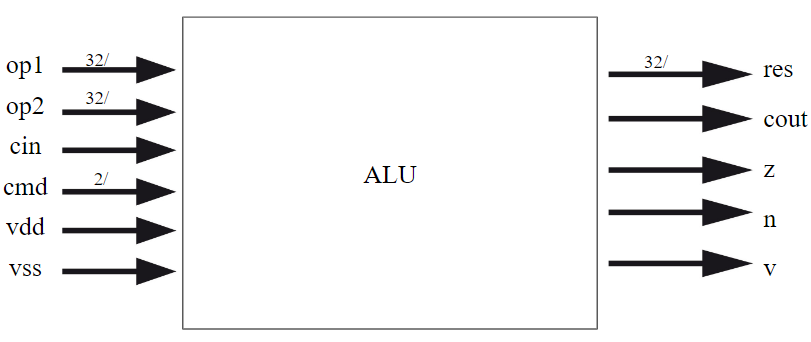
\includegraphics[width=0.9\textwidth]{alu.png} 							%[]size,{}nom
				\caption{Schéma bloc de l'Alu} 													%titre de figure
				\label{Fig.main2} 														%label interne
			\end{figure}

			L'Alu est le composant qui nous permet de réaliser les 4 opérations de base : ADD avec retenue, 
			AND, OR et XOR. Mais afin de sélectionner l'opération voulue entre les deux opérandes de 32 bits, 
			nous utilisons une commande sur deux bits. Les opérations AND, OR et XOR sont très simples à 
			implémenter à l'aide des opérateurs qui sont déjà mis à disposition. Cependant, pour l'opération 
			d'addition, nous avons utilisé un Full Adder en l'instanciant 32 fois. Lors de la synthèse nous 						avons constaté que l'instanciation avec un seul "generate (de 0 à 31)" génère une erreur sur les 
			retenues car les retenues 1 à 31 ne sont pas assignées. En effet, nous avons dû réaliser une
			première instanciation pour produire le résultat de rang 0, ensuite l'instanciation avec un
			generate de 1 à 30 et une dernière instanciation pour produire le résultat de rang 31.
			
			\begin{figure}[H]															%à cette position 
				\centering 																%au milieu 
				\includegraphics[width=1.0\textwidth]{alu_detaille.png} 				%[]size,{}nom
				\caption{Schéma des opérations réalisés par l'Alu} 						%titre de figure
				\label{Fig.main2} 														%label interne
			\end{figure}
			
			\newpage
			
			\begin{figure}[H]															%à cette position 
				\centering 																%au milieu 
				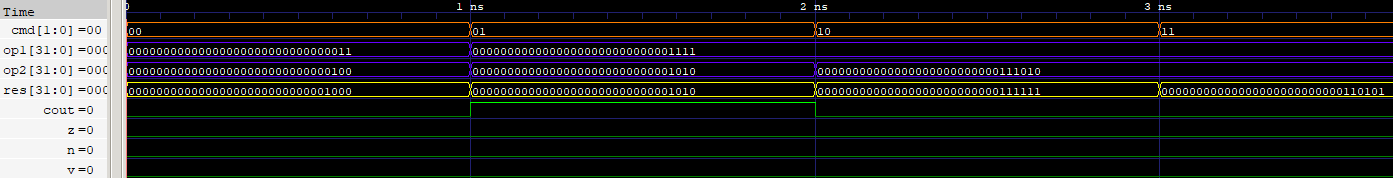
\includegraphics[width=1.0\textwidth]{alu_gtkwave.png}					%titre de figure
				\caption{Résultat de simulation pour l'Alu} 							%titre de figure
				\label{Fig.main2} 														%label interne
			\end{figure}
			
			La figure ci-dessus illustre le bon fonctionnement de l’alu. En effet, les opérations suivantes 
			sont réalisées dans l’ordre add, and, or et xor en fonction de la commande sur 2 bits . 

%			%parameter values era given in Table \ref{tab:tab2}.
%			\begin{table}[H]
%				\centering
%				\begin{tabular}{|c|c|}
%					\hline
%					cmd & Opération \\\hline
%					00 & ADD \\
%					01 & OR \\
%					10 & AND \\
%					11 & XOR \\
%					\hline
%				\end{tabular}
%				\caption{}\label{tab:tab2}
%			\end{table}
			
			Dans ce projet nous réalisons la synthèse en 3 étapes en utilisant 3 logiciels de la suite alliance. 
			Tout d’abord avec vasy nous réalisons une conversion .vhdl en .vbe afin d’obtenir des structures 
			simples. Puis avec boom nous réalisons une optimisation booléenne donc nous avons toujours un .vbe. 
			Enfin, avec boog nous réalisons une projection structurelle afin de convertir les équations en 
			netlist de portes logiques. Afin d’illustrer ces 3 étapes nous pouvons nous appuyer sur un exemple 
			très simple qui est le premier composant du projet, le Full Adder.
		
			\begin{figure}[H]															%à cette position 
				\centering 																%au milieu 
				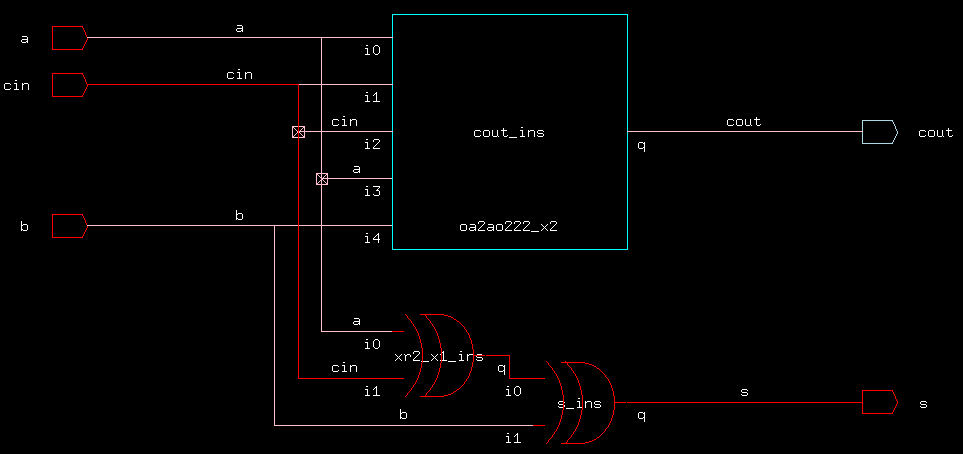
\includegraphics[width=0.9\textwidth]{full_adder_XSCH.png} 				%[]size,{}nom
				\caption{Résultat de synthèse pour le Full Adder} 						%titre de figure
				\label{Fig.main2} 														%label interne
			\end{figure}

			cout = (A and B) or (Cin and B) or (A and Cin) = A and (B or Cin) or (B and Cin) 
			%\\ \hspace*{\fill} \\														%une ligne d'espace 
			Pour la sortie s on s'attend à obtenir le schéma en portes logiques suivant A xor B xor Cin, cela 
			est cohérent avec le résultat de synthèse. Cependant pour la sortie cout on s'attendait à obtenir 
			(A and B) or (Cin and B) or (A and Cin) (1) soit un oa23\_x2 dans la terminologie sxlib, 
			mais le bloc de synthèse correspond à un oa2ao222\_x2, on remarque que cela correspond à 
			l'équation logique suivante A and (B or Cin) or (B and Cin). On en déduit qu'il s'agit juste 
			d'une optimisation de l'équation (1) réalisée par boom car le A a été mis en facteur. On peut 
			également remarquer que la synthèse présente un chemin rouge, ce-dernier représente le chemin 
			critique c'est-à-dire le chemin le plus long du composant.
			
			\begin{figure}[H]															%à cette position 
				\centering 																%au milieu 
				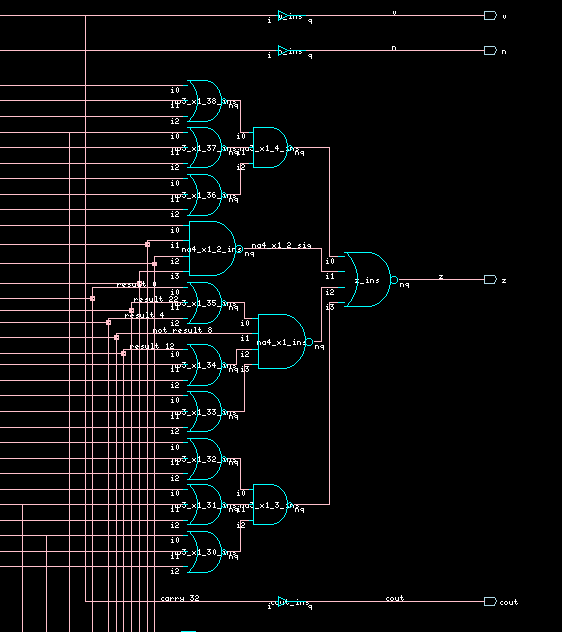
\includegraphics[width=0.9\textwidth]{alu_cznv_XSCH.png} 				%[]size,{}nom
				\caption{Résultat de synthèse pour l'Alu (zoom sur la génération des flags czn et v)}
				\label{Fig.main2} 														%label interne
			\end{figure}
			
			\begin{itemize}															%signe [(1)]
				\item c : retenue de sortie
				\item z : résultat nul
				\item n : résultat négatif 
				\item v : dépassement de capacité
			\end{itemize}

			\begin{figure}[H]															%à cette position 
				\centering 																%au milieu 
				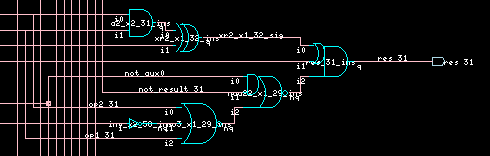
\includegraphics[width=0.9\textwidth]{alu_res_XSCH.png} 				%[]size,{}nom
				\caption{Résultat de synthèse pour l'Alu (zoom sur le bit 31 du vecteur res)}%titre de figure
				\label{Fig.main2} 														%label interne
			\end{figure}
			
			Le vecteur res correspond à la sortie de l'alu sur 32 bits et le schéma en portes logiques 
			des bits de rang inférieur reste identique à celui représenté sur la figure.

		%%%%%%%%%%%%%%%%%%%%%%%%%%%%%%%%%%%%%%%%%%%%%%Shifter%%%%%%%%%%%%%%%%%%%%%%%%%%%%%%%%%%%%%%
		\subsection{Shifter}															%sous titre shifter
			\begin{figure}[H]															%à cette position 
				\centering 																%au milieu 
				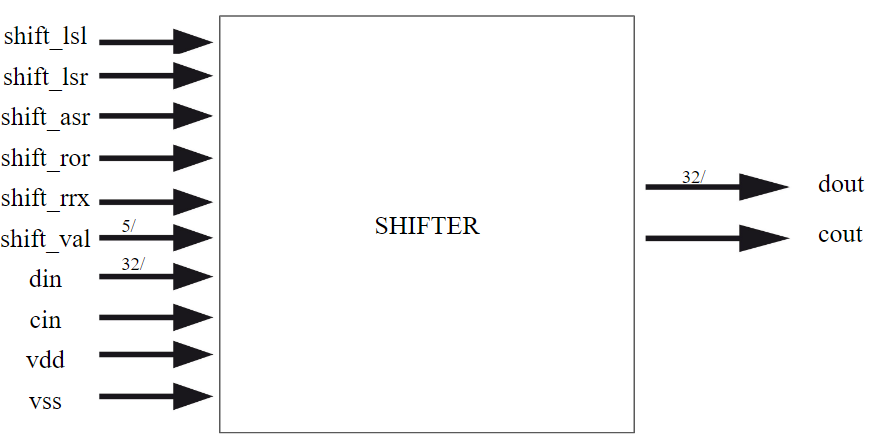
\includegraphics[width=0.8\textwidth]{shifter.png} 						%[]size,{}nom
				\caption{Schéma bloc du Shifter}												%titre de figure
				\label{Fig.main2} 														%label interne
			\end{figure}
			
			Un autre composant essentiel pour notre processeur ARM est le shifter. En effet, 
			ce-dernier nous permet de réaliser des décalages et rotations. La technique employée consiste à 
			réaliser des décalages ou des rotations progressifs. La valeur de décalage étant définie par une 
			valeur binaire sur cinq bits, nous pouvons décomposer l'opération en des décalages de $2^N$  avec
			N=0, 1, 2, 3 et 4. Ainsi, chaque valeur de décalage comprise entre 0 et 31 peut être réalisée. 
			On comprend donc que nous réalisons des concaténations de 0 ou 1 en fonction de s'il s'agit 
			d'un décalage logique ou arithmétique. 
			
			\subsubsection{Décalages logiques}												%sous titre decalage
	         	Pour les décalages logiques : Logic shift left(LSL) et Logic shift right(LSR) 
				nous réalisons simplement des concaténations de 0. 
				
				\begin{figure}[H]															%à cette position 
					\centering 																%au milieu 
					\includegraphics[width=0.95\textwidth]{shifter_lsl_lsr.png}				%[]size,{}nom
					\caption{Décalages logiques shift left(LSL) et shift right(LSR) }		%titre de figure
					\label{Fig.main2} 														%label interne
				\end{figure}

			\subsubsection{Décalage arithmétique vers la droite}							%sous titre decalage
				Cependant, dans le cas d'un décalage arithmétique vers la droite : 
				arithmetic shift right(ASR) nous devons tenir compte du bit de signe pour la concaténation.

				\begin{figure}[H]															%à cette position 
					\centering 																%au milieu 
					\includegraphics[width=0.95\textwidth]{shifter_asr.png} 				%[]size,{}nom
					\caption{Décalage arithmétique vers la droite (ASR)}%titre de figure
					\label{Fig.main2} 														%label interne
				\end{figure}

			\subsubsection{Rotation vers la droite}											%sous titre decalage
				Dans le cas d’une rotation nous utilisons directement les bits de notre opérande pour réaliser 
				la concaténation.   
				
				\begin{figure}[H]															%à cette position 
					\centering 																%au milieu 
					\includegraphics[width=0.95\textwidth]{shifter_ror.png} 				%[]size,{}nom
					\caption{Rotation vers la droite (ROR)}%titre de figure
					\label{Fig.main2} 														%label interne
				\end{figure}
			\subsubsection{Rotation vers la droite avec étendue}							%sous titre decalage
				Pour la rotation vers la droite avec étendue nous réalisons une seule concaténation avec la 
				retenue d’entrée.

				\begin{figure}[H]															%à cette position 
					\centering 																%au milieu 
					\includegraphics[width=0.95\textwidth]{shifter_rrx.png} 				%[]size,{}nom
					\caption{Rotation vers la droite avec étendue (RRX)}%titre de figure
					\label{Fig.main2} 														%label interne
				\end{figure}
			%Le principe de ces décalages est présenté sur la figure ci-dessous.
			
			\begin{figure}[H]															%à cette position 
				\centering 																%au milieu 
				\includegraphics[width=1.0\textwidth]{shifter_detaille.png} 			%[]size,{}nom
				\caption{Le principe des décalages}										%titre de figure
				\label{Fig.main2} 														%label interne
			\end{figure}
			La figure ci-dessus illustre les différents décalages en fonction de l'état binaire de shift\_lsl, 
			shift\_lsr, shift\_asr, shift\_ror et shift\_rrx. Nous réalisons un décalage de $2^n$ bits lorsque 
			le bit de rang n du vecteur shift\_val est à 1. Le bit din(31) est utilisé pour réaliser une 
			extension de signe dans le cas où l'on souhaite réaliser un ASR.

			\begin{figure}[H]															%à cette position 
				\centering 																%au milieu 
				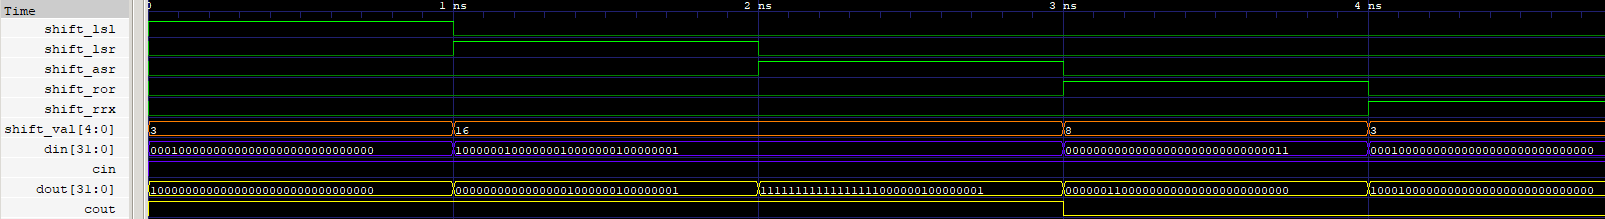
\includegraphics[width=1.0\textwidth]{shifter_gtkwave.png} 				%[]size,{}nom
				\caption{Résultat de simulation pour le shifter}						%titre de figure
				\label{Fig.main2} 														%label interne
			\end{figure}
			Afin de vérifier le bon fonctionnement du shifter, nous réalisons les 5 décalages possibles. 
			Dans la réalisation de ce composant il a fallu particulièrement faire attention à réaliser 
			correctement l'extension de signe dans le cas d’un décalage arithmétique et de correctement 
			identifier la retenue de sortie en fonction du type de décalage car elle vaut dout(31) dans le cas 
			d'un LSL et dout(0) sinon (LSR, ASR, ROR et RRX).
	\newpage
	
	%%%%%%%%%%%%%%%%%%%%%%%%%%%%%%%%%%%%%%%%%%%%%%Decode%%%%%%%%%%%%%%%%%%%%%%%%%%%%%%%%%%%%%%
	\section{Étage Decod}                      								%——titre Decode
		\subsection{Le banc de registre}
			\begin{figure}[H]															%à cette position 
				\centering 																%au milieu 
				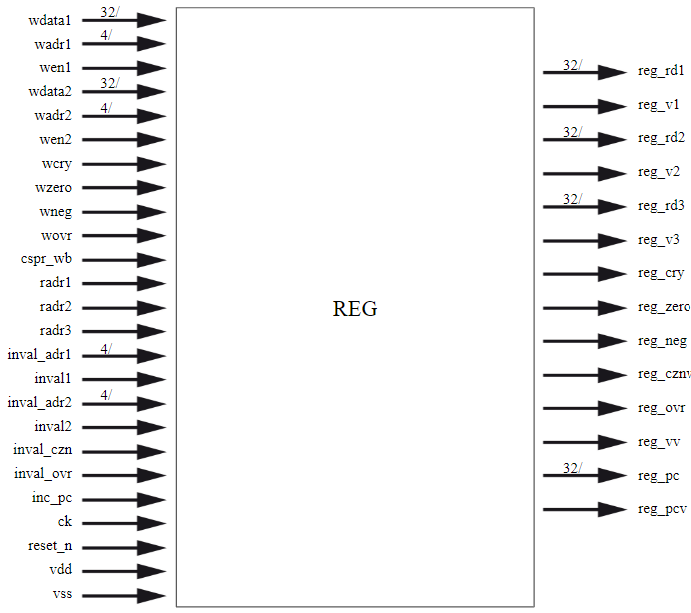
\includegraphics[width=0.8\textwidth]{reg.png} 							%[]size,{}nom
				\caption{Schéma bloc de reg}											%titre de figure
				\label{Fig.main2} 														%label interne
			\end{figure}
			
			L'étage decod est l'étage le plus complexe du processeur car ce dernier est chargé de décoder les 
			instructions de l'architecture ARM... . En effet, il existe différents types d'instructions et ces 
			dernières utilisent des opérandes sur 32 bits, il convient d'utiliser des registres pour ces 
			opérandes et pour cela nous avons utilisé un bloc appelé reg. Ce bloc contient :
			
			\begin{itemize}															%signe [(1)]
				\item 3 ports de lecture numérotés de 1 à 3,
				\item 2 ports d’écriture, le numéro 1 correspond à exec et est donc prioritaire,
				\item 2 ports d’invalidation car une instruction peut produire 2 résultats,
				\item 4 flags : c,z,n,v et leurs 2 bits de validité (1 bit de validité pour czn et 1 pour ovr),
				\item PC, son bit de validité et sa commande de +4
			\end{itemize}
			
			Pour le banc de registre nous avons décidé de réaliser un process synchrone qui est sensible sur 
			l'horloge(ck) et reset\_n pour l'écriture dans les registres et la gestion des bits de validité 
			associés, la mise à jour des flags et la gestion des bits de validité associés, enfin la gestion de 
			pc (incrémentation de 4). Au reset tous les bits de validité sont initialisés à ‘1’. Cependant, 
			pour la lecture nous avons décidé de la réaliser en concurrent. Pour l'écriture lorsqu'un registre 
			est identifié comme une destination, ce dernier est invalidé, pour cela une solution est d'utiliser 
			un vecteur invalid dont le bit de rang n indique s'il est égal à 1 que le registre n est invalidé. 
			Lorsque l'écriture a été effectuée, le registre est à nouveau validé. Afin de gérer la priorité 
			entre le port 1 et 2, nous avons créé 2 autres vecteurs wadr1\_v et wadr2\_v, lorsque l'on souhaite 
			écrire dans le registre n via le port 1 il faut que wadr1\_v(n) soit à 1, cependant lorsque l'on 
			veut écrire dans le registre n via le port 2 il faut que wadr2\_v(n) soit à 1 et wadr1\_v(n) à 0. 
			
			\begin{figure}[H]															%à cette position 
				\centering 																%au milieu 
				\includegraphics[width=0.9\textwidth]{reg_detaille.png} 				%[]size,{}nom
				\caption{Schéma global de reg}											%titre de figure
				\label{Fig.main2} 														%label interne
			\end{figure}

			La figure ci-dessus illustre le principe de fonctionnement du banc de registre pour un registre 
			précis mais le principe reste le même pour les 15 autres registres. En effet, ici nous utilisons un 
			exemple où le registre 15 (PC) est la destination d’une écriture via le port 1 et 2, cela nous 
			permet de montrer la prise en compte de la priorisation du port 1 lorsque l'adresse du registre de 
			destination est la même pour les 2 écritures.
 			
			\begin{figure}[H]															%à cette position 
				\centering 																%au milieu 
				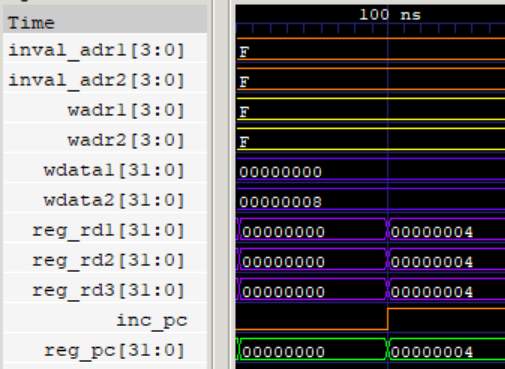
\includegraphics[width=0.6\textwidth]{reg_gtkwave.png}					%[]size,{}nom
				\caption{Résultat de simulation pour le banc de registre}				%titre de figure
				\label{Fig.main2} 														%label interne
			\end{figure}

			Le résultat de simulation ci-dessus, nous montre que pour une même adresse de destination qui est 
			le registre PC ici, la donnée est écrite via le port 1. En effet, ici les 3 ports de lecture lisent 
			le même registre (PC) et nous voyons bien que la valeur lue correspond à celle de wdata1 et non 
			wdata2. Enfin, nous avons testé l'incrémentation du registre pc, nous remarquons qu'elle se fait 
			bien lorsque inc\_pc vaut 1. 
		
			\begin{figure}[H]															%à cette position 
				\centering 																%au milieu 
				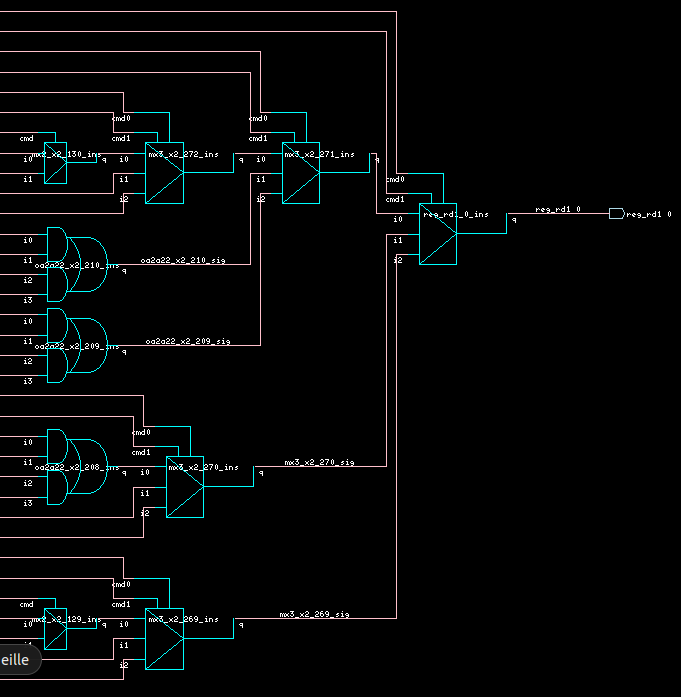
\includegraphics[width=1.0\textwidth]{reg_rd1(0).png} 					%[]size,{}nom
				\caption{Résultat de synthèse pour le banc de registre  (zoom sur le port de lecture 1)}
				\label{Fig.main2} 														%label interne
			\end{figure}

			\begin{figure}[H]															%à cette position 
				\centering 																%au milieu 
				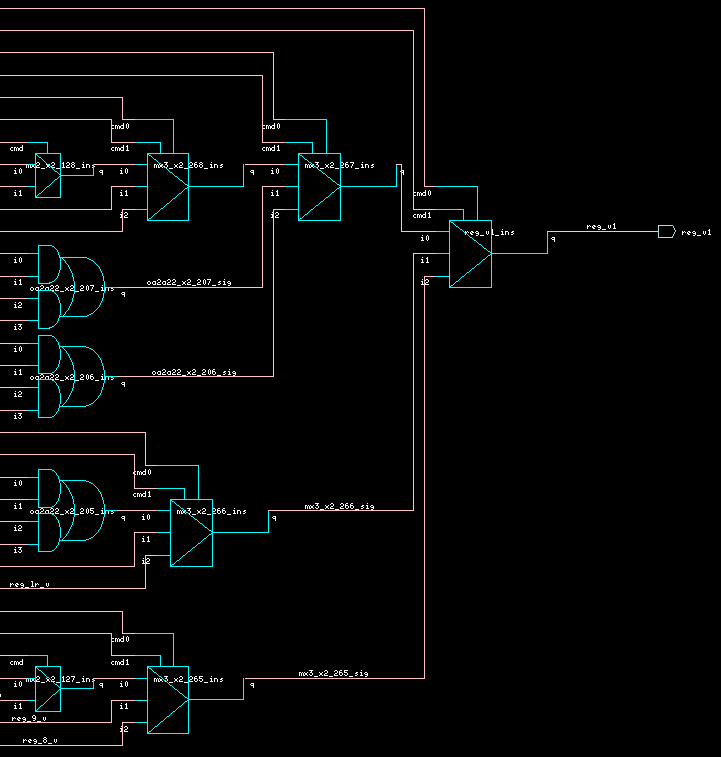
\includegraphics[width=1.0\textwidth]{reg_v1.png} 						%[]size,{}nom
				\caption{Résultat de synthèse pour le banc de registre  (zoom sur la gestion du bit de validité 							du port de lecture 1)}
				\label{Fig.main2} 														%label interne
			\end{figure}

			\begin{figure}[H]															%à cette position 
				\centering 																%au milieu 
				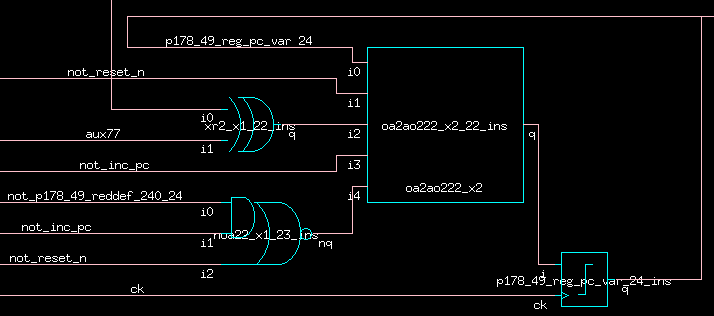
\includegraphics[width=1.0\textwidth]{+4_pc.png} 							%[]size,{}nom
				\caption{Résultat de synthèse pour le banc de registre  (zoom sur la gestion de PC)}
				\label{Fig.main2} 														%label interne
			\end{figure}
\end{document}

